\documentclass[11pt, a4paper, USenglish]{article} % change ``USenglish'' to ``norsk'' if applicable.

\usepackage{kyblab} % Contains all included packages. See kyblab.sty.
\addbibresource{bibliography.bib} % Makes the bibliography file available to biblatex.

\begin{document}

% Titlepage
\title{LaTeX Lab Report Template}
\author{Group 61\\Student Kenny Hoang Nguyen 478374\\Student Martin Lund Haug xxxxx\\}
\date{April, 2020}
\begin{titlepage}
    \maketitle
    \begin{figure}
    \centering
    
\includegraphics[width=0.5\textwidth]{figures/logontnu_eng.pdf}\\
    \end{figure}
    \thispagestyle{empty}
\end{titlepage}

% Abstract
\newpage
\begin{abstract}
In this project a detector is derived using knowledge about the statistic distribution to the signals that needs to be detected which are drowned in noise.
The exact detector is derived for this specific problem, then an approximate detector is used for better performance. 
A short summary using about half a page about:
\begin{enumerate}[i]
    \item The course/project
    \item the results
    \item conclusion
\end{enumerate}
\end{abstract}
\thispagestyle{empty} % Avoid page numbering on the summary page.

% TOC
\newpage
\tableofcontents
\thispagestyle{empty} % Avoid page numbering on the table of contents.

% Main content
\newpage
\setcounter{page}{1}
\section{Introduction}\label{sec:intro}
Here we should write about
\begin{enumerate}[i]
	\item The goals/motivation of the course/project.
	\item Why is your task of general interest to society? etc\dots
	\item How the report is organized
	\begin{itemize}
		\item In chapter x the theory is described
		\item in chapter y the implementation is described
		\item \dots
		\item and finally the conclusion is given in chapter z
	\end{itemize}
\end{enumerate}

You cite by using \cite{Chen2014}
\section{Theory}\label{sec:theory}
\subsection{Gaussian Distribution}
The gaussian distribution or the normal distribution is an important distribution that is often used in natural and social sciences for real-valued random variables when their distributions are not known. The importance of this distribution comes from the central limit theorem, that states for any under some conditions the average of many (enough) observations of a random variable with finite mean and variance converges to a normal distribution even if the random variable comes from another distribution.\cite{WikipediaGaussian}. The most important thing here is that the probability density function of a normal distribution with mean $\mu$ and variance $\sigma^2$ is
\begin{equation}
	f(x) = \frac{1}{\sqrt{2\pi\sigma^2}}e^{-\frac{1}{2}(\frac{x-\mu}{\sigma})^2}
\end{equation}
which gives the probability to obtain any value $x\in\mathbb{R}$ from this distribution.\\
In this particular project we use the complex gaussian distribution which for our random variables has the probability density function
\begin{equation}
	f(x) = \frac{1}{\pi\sigma^2}e^{-\frac{1}{\sigma^2}|x-\mu|^2}
\end{equation}
Which in this case take in any value $x\in\mathbb{C}$.
\subsection{$\chi^2$ distribution}
In this project the $\chi^2$ distribution is also an important distribution that is going to be used. The reason for this is because it has a more approachable point distribution function that is easier to handle when finding the cumulative distribution of a square normal distribution. The most important property of the $\chi^2$ is that it is the distribution of a sum of the squares of a $k$ independent standard normal variables with $k$ degrees of freedom.\cite{WikipediaChi}
\subsection{Estimators}
When we with probable cause can say something about the distribution that the random variables are sampled from, but not their mean and/or variance, we can estimate these distributions properties. Assumed that the random variables are sampled independent from the same identical distribution (iid), then the mean can be estimated with the average of the samples, which is unbiased.
\begin{align}
	\hat{\mu} & = \mathbb{E}\{\frac{1}{N}\sum_{n=0}^{N-1}x\}\nonumber\\
	& = \frac{1}{N}\sum_{n=0}^{N-1}\mathbb{E}\{x\}\nonumber\\
	& = \frac{1}{N}\sum_{n=0}^{N-1}\mu\nonumber\\
	& = \mu\label{eq:mu_est}
\end{align}
Meaning that the expected value of the mean of the samples will, with the number of samples taken, converge to the actual expected value of the distribution.\\
This is also the case if there are samples of the variance of the data available
\begin{align}
	\hat{\sigma^2} & = \mathbb{E}\{\frac{1}{N}\sum_{n=0}^{N-1}\sigma^2\}\nonumber\\
	& = \frac{1}{N}N\sigma^2\nonumber\\
	& = \sigma^2\label{eq:sigma_est}
\end{align}
These two results are used when solving the problems later on in this report.
\subsection{(Binary) Hypothesis Testing}
Detection problems are often formulated to be about if a signal is present or not in conditions which masks the signal that we desire to detect, for instance white gaussian noise. The hypothesises that could be formulated is:
\begin{align}
\begin{split}
	\text{Null hypothesis} H_0 &: x[n] \thicksim \mathbb{P}_0\\
	\text{Alternative hypothesis} H_1 &: x[n] \thicksim \mathbb{P}_1
\end{split}
\end{align}\label{eq:gen_hypothesis_test}
where the null hypothesis is ''no signal present'' and alternative hypothesis is ''signal present'', and $\mathbb{P}_0$ and $\mathbb{P}_1$ are two arbitrary distributions.\\
Let $[x[0] x[1] \dots x[N-1]]$ be sampled random variables from a sensor where it is constant "1" when detecting an object and constant "0" when not detecting anything. A simple detector in this case could be by setting a threshold at $\lambda = 0.3$ that detects when the threshold is broken. The problem with this simple detector appears when the signal from our sensor is noisy.\\
Let now the samples from our sensor be
\begin{align}
	H_0 &: x[n] = w[n]\nonumber\\
	H_1 &: x[n] = A + w[n]\nonumber
\end{align}
where $w[n] ~ \mathcal{N}(0, 1)$. Then under the null hypothesis in a non-noisy environment $w[n] = 0 \implies x[n] = 0$, however we have a noisy envirnoment so $x[n]$ obtains random values from the normal distribution with zero mean and unit variance. In figure \ref{fig:noise} we can see how the data we obtain from 100 samples may look like.
\begin{figure}
	\centering
	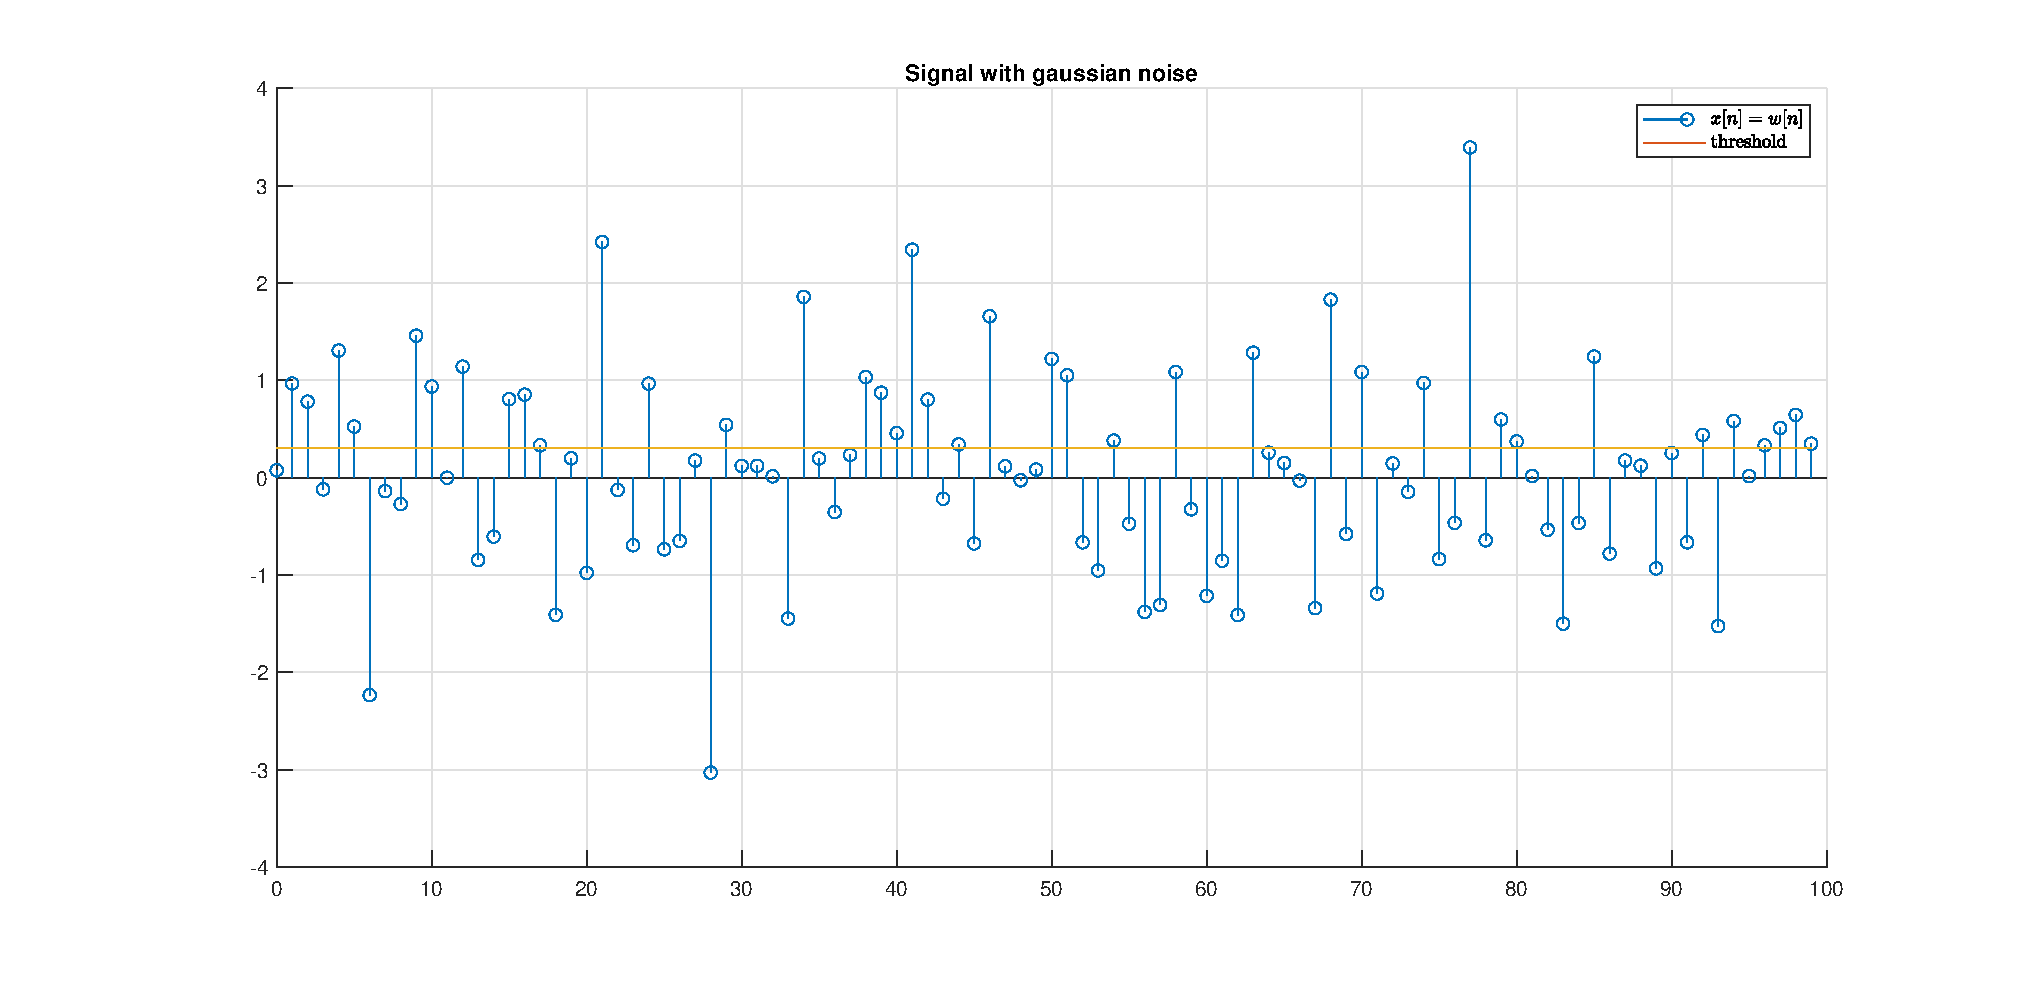
\includegraphics[width = \linewidth]{figures/gen_sign_noise.eps}
	\caption{100 samples from a gaussian distribution $\mathcal{N}(0,1)$}
	\label{fig:noise}
\end{figure}
From these 100 samples there are 39 samples that are above the set threshold meaning that from these 100 samples we will get 39 false positives/alarms which will alert the user that there is an object detected when there really is not. Our goal when solving detection problems is to develop a detector that from the samples can find a decision rule so that the number of false alarms is minimized but at the same time manages to detect correctly when there is an object present.\cite{Myrvoll2020}\\
\subsection{Neyman-Pearson detector}
The Neyman-Pearson detector utilizes the likelihood ratio test (LRT)
\begin{equation}
	L(\mathbf{x}) \triangleq \frac{p_1(\mathbf{x})}{p_0(\mathbf{x})} 
		\begin{cases}
			\geq \lambda \implies H_1
			< \lambda \implies H_0
		\end{cases} 
\end{equation}
where $p_1(x)$ and $p_0(x)$ is the point distribution functions or the likelihood functions of the distributions under $H_1$ and $H_0$ respectively.
With the Neyman-Pearson detector the threshold $\lambda$ is chosen to satisfy the constraint and to maximize the power such that
\begin{equation}
	P_{FA} = \alpha = \int_{L(\mathbf{x})>\lambda}p_0(\mathbf{x})d\mathbf{x}
\end{equation}
where $\alpha_0$ the tuning factor. This goes hand in hand with the detection rate of the detector as well since the Neyman-pearson lemma states that to increase the power of the likelihood ratio test, the false alarm rate is also increased. \todo{Mye dårlige formuleringer her. Må skrives om}
\begin{enumerate}[i]
	\item \underline{Inform} the reader that this chapter is a presentation of the theory needed to understand the task
	\item You may copy parts from lecture notes (but inform
	the reader that you have done this!). Also refer to
	books in former courses or other literature
	\begin{itemize}
		\item Always refer to the source and
		\item Use quotation marks when quoting (copying) 
	\end{itemize}
	\item Use figures if possible/natural!
\end{enumerate}
\section{The tasks}\label{sec:task}
The main problem that is going to be solved in this project is the detection problem
\begin{align}
\begin{split}
	H_0: x(n) & = w(n), n = 0, 1, \dots, N-1\\
	H_1: x(n) & = s(n) + w(n), n = 0, 1, \dots, N-1
\end{split}
\end{align}\label{eq:detection_problem}
where $s(n)$ is a waveform sequence of the PU and $w(n)$ is an additive white complex Gaussian noise.
To construct the sequence $s(n)$, that is transmitted over the wireless channel, the modulation method orthogonal frequency-division multiplexing (OFDM) is used. Each information symbol $S(k)$, $k=0,1,\dots,N-1$ is allocated on each N carrier frequencies. The unique time-domain signal $s(n)$ corresponding to the sampled spectrum is obtained by inverse discrete Fourier transform. Thus is the PUs time-domain signal given by:
\begin{equation}
	s(n) = \frac{1}{\sqrt{N}}\sum_{k=0}^{N-1}S(k)e^{\frac{j2\pi nk}{N}}, n = 0,1,\dots,N-1
\end{equation}
which we notice is a complex-valued quantity.

\subsection{Task 1: Model building}
Here the data $x[n]$ is generated, which can be used in our analysis to obtain a suitable detector. To generate $x[n]$ we need do to verify that the complex-valued time-domain OFDM signal sequence $s(n) = s_R(n)+js_I(n)$ is independent and identically distributed, in addition to verify that it is accurately modelled with a complex Gaussian distribution.\\
The data sets T1 are used, they contain samples that are taken from a standard normal Gaussian distribution and binary phase shift keying respectively.

\subsection{Task 2: One-sample detector}
In this task only a single sample is used to generate the NP-detector. That is, there needs to be done calculations to retrieve the decision rule that decides for when to choose null hypothesis over the alternative hypothesis and vice versa.

\subsection{Task 3: Performance of the one-sample detector}
Here the data sets T3 are given and are to be used to verify that
\begin{align}
	H_0 &: \frac{2x_R^2(0)}{\sigma_w^2}+\frac{2x_I^2(0)}{\sigma_w^2}=\frac{2|x(0)|^2}{\sigma_w^2}\label{eq:chi_sq_h0}\\
	H_1 &: \frac{2x_R^2(0)}{\sigma_w^2+\sigma_s^2}+\frac{2x_I^2(0)}{\sigma_w^2+\sigma_s^2}=\frac{2|x(0)|^2}{\sigma_w^2+\sigma_s^2}\label{eq:chi_sq_h1}
\end{align}
are $\chi^2$-distributed with 2 degrees of freedom. This can be used to show that $\widetilde{x} = \frac{2|x(0)|^2}{\sigma^2}$ has the point-distribution function $f(\widetilde{x}) = \frac{1}{2}e^{-\frac{\widetilde{x}}{2}}$ for $\widetilde{x}>0$. Further, the result can then be used to calculate the probability for false alarm and the probability for detection for this one-sample detector.

\subsection{Task 4: General NP detector}
In this task the one-sample detector derived in the previous tasks are generalized so it can be used when there are $K>1$ samples. Since $|x(n)|^2$ is a sum of two standard normal Gaussian squared, then in the case where there are multiple samples, the $\chi^2$-distribution has $2K$ degrees of freedom which can be used to derive the threshold $\lambda'$ that maximizes $P_D$ and ensure that $P_{FA}<\alpha$.

\todo{Task 5-8 needs to be rewritten/reformulated}
\subsection{Task 5: Performance of the general NP detector}
In this task the distribution obtained in task 4 is used to plot the receiver operating characteristics.

\subsection{Task 6: Approximate performance of the general NP detector}
Here the central limit theorem is used to approximate the test statistic. The PDF of the test statistic is calculated, and thus can $P_D$ and $P_{FA}$ be plotted as a function of the threshold where the Gaussian is used instead of the pdf from the gamma distribution.

\subsection{Task 7: Complexity of the detector}
In the former task the detector was approximated to be from the Gaussian distribution. Using this knowledge, an expression for how many samples that are needed to attain a given $P_D$ and $P_{FA}$ is derived.

\subsection{Task 8: Numerical experiments in PU detection}
The NP detector that has been found is used on a numerical experimental data that contains 100 realizations of a PU signal. The task is to see if the detector will detect the PU.
\section{Implementation and results}\label{sec:results}
\subsection{Task 1: Model development}\todo{Vi må muligens flytte mye av dette over til "tasks" delen. Prøve å bare ha resultater her og ikke utregninger? Enig/ikke enig?}
\begin{figure}[ht]
    \begin{subfigure}{.5\textwidth}
        \centering
        % include first image
        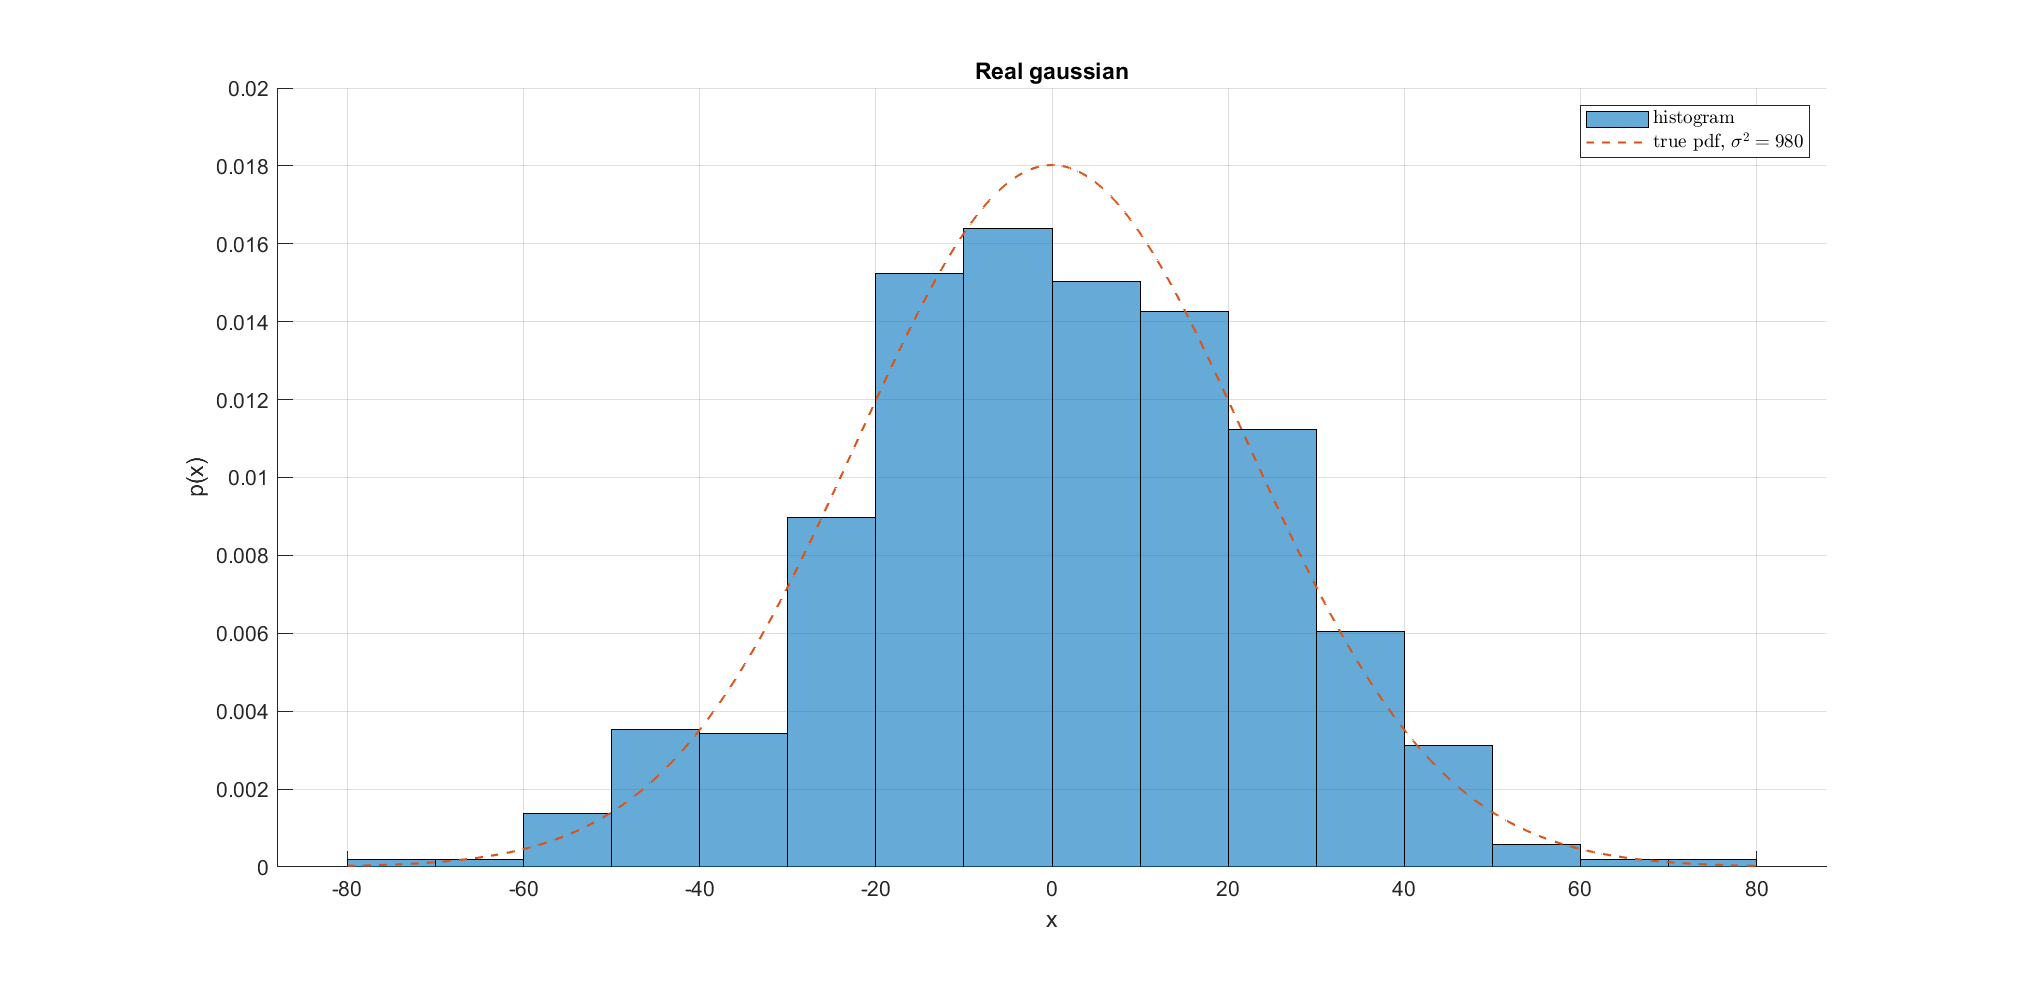
\includegraphics[width=.8\linewidth]{figures/re_gauss.eps}  
        \caption{The histogram of Re(S(k))$~$Gaussian}
        \label{fig:re_gauss}
    \end{subfigure}
    \begin{subfigure}{.5\textwidth}
        \centering
        % include second image
        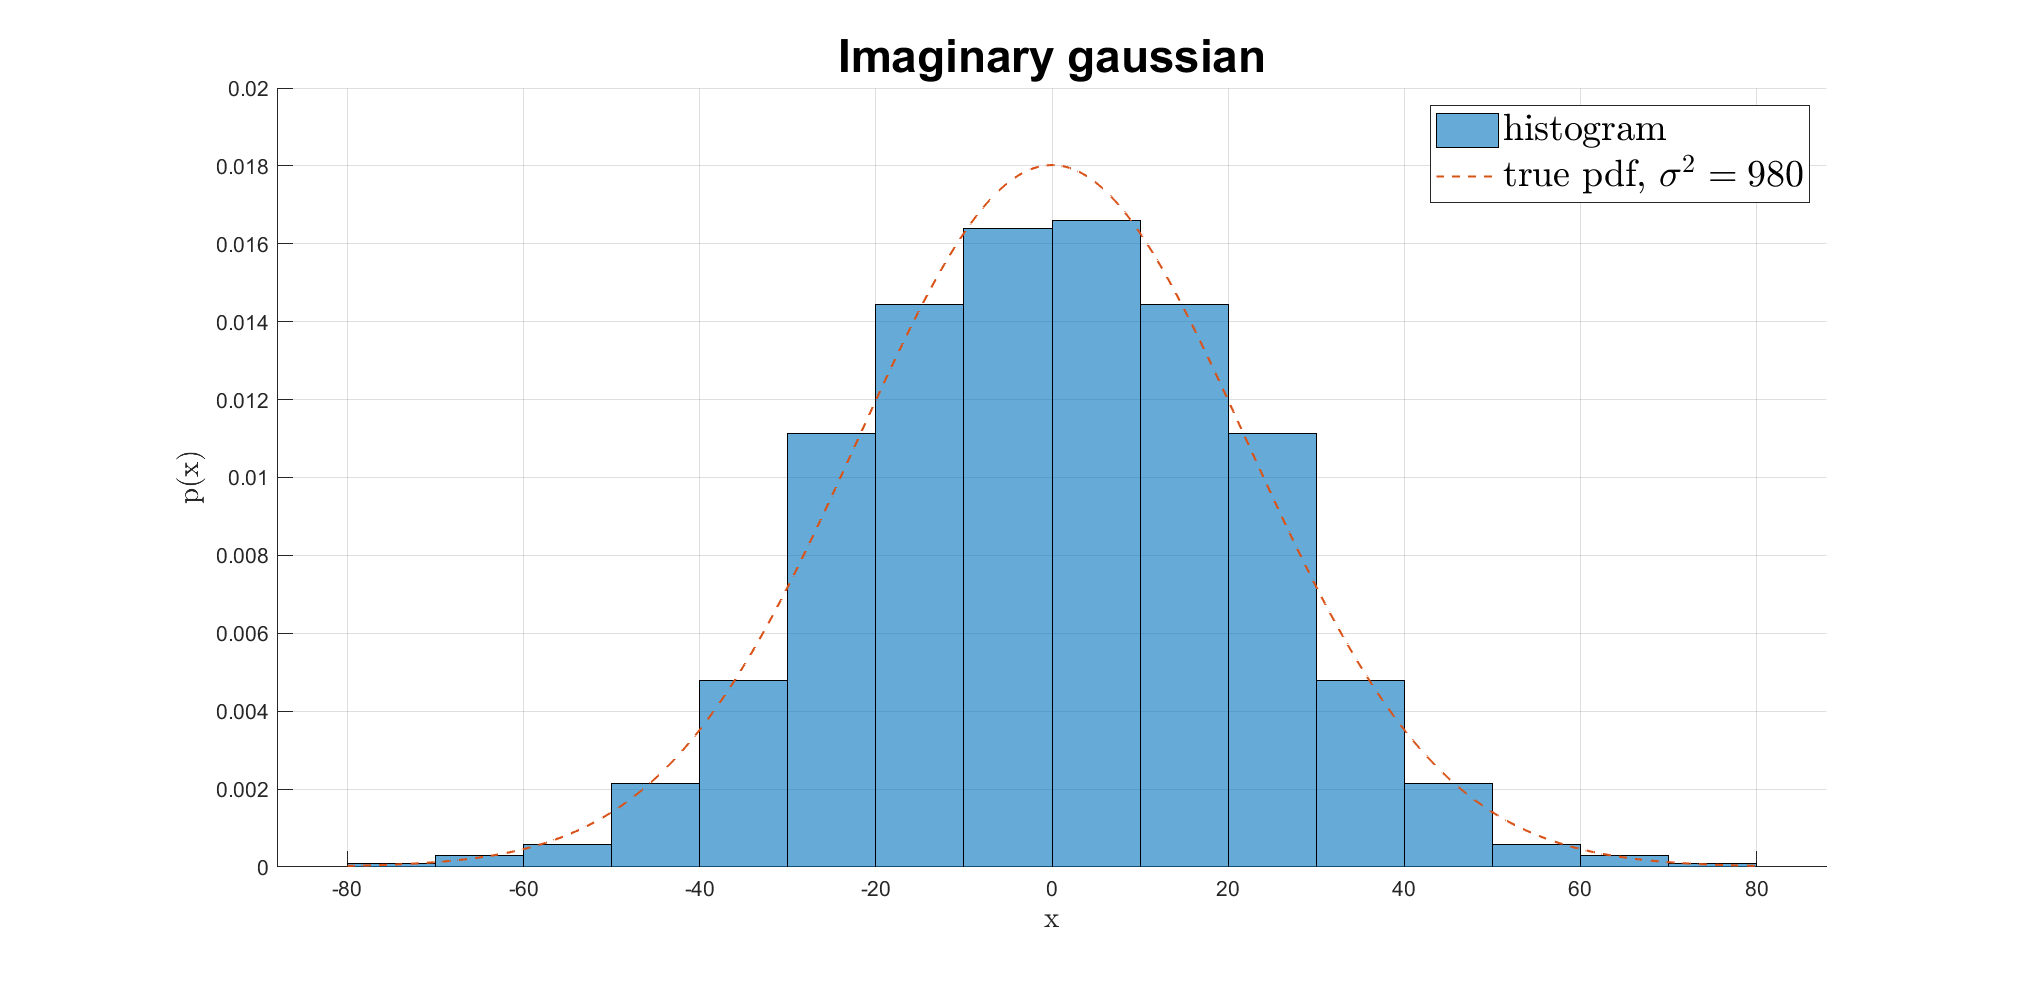
\includegraphics[width=.8\linewidth]{figures/im_gauss.eps}  
        \caption{The histogram of Im(S(k))$~$Gaussian}
        \label{fig:im_gauss}
    \end{subfigure}
    \begin{subfigure}{.5\textwidth}
        \centering
        % include third image
        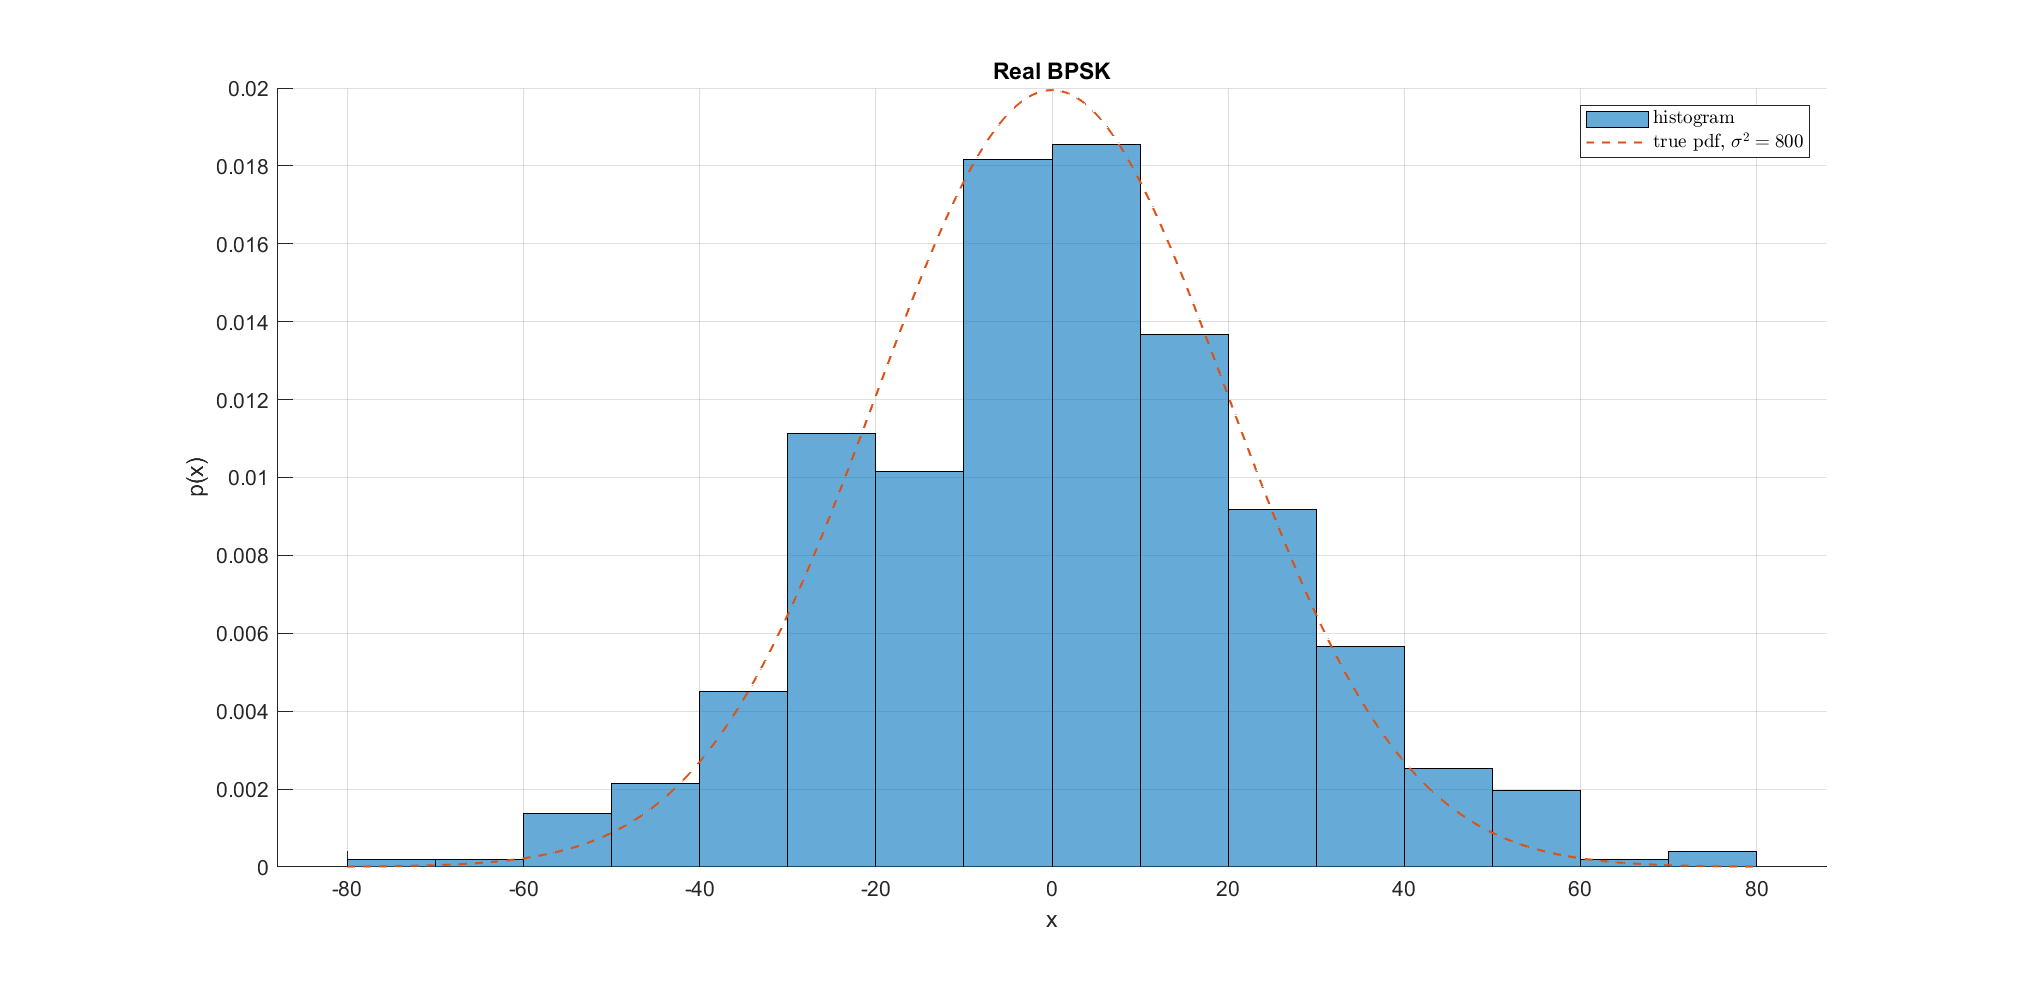
\includegraphics[width=.8\linewidth]{figures/re_bpsk.eps}
        \caption{The histogram of Re(S(k))$~$BPSK}
        \label{fig:re_bpsk}
    \end{subfigure}
    \begin{subfigure}{.5\textwidth}
        \centering
        % include fourth image
        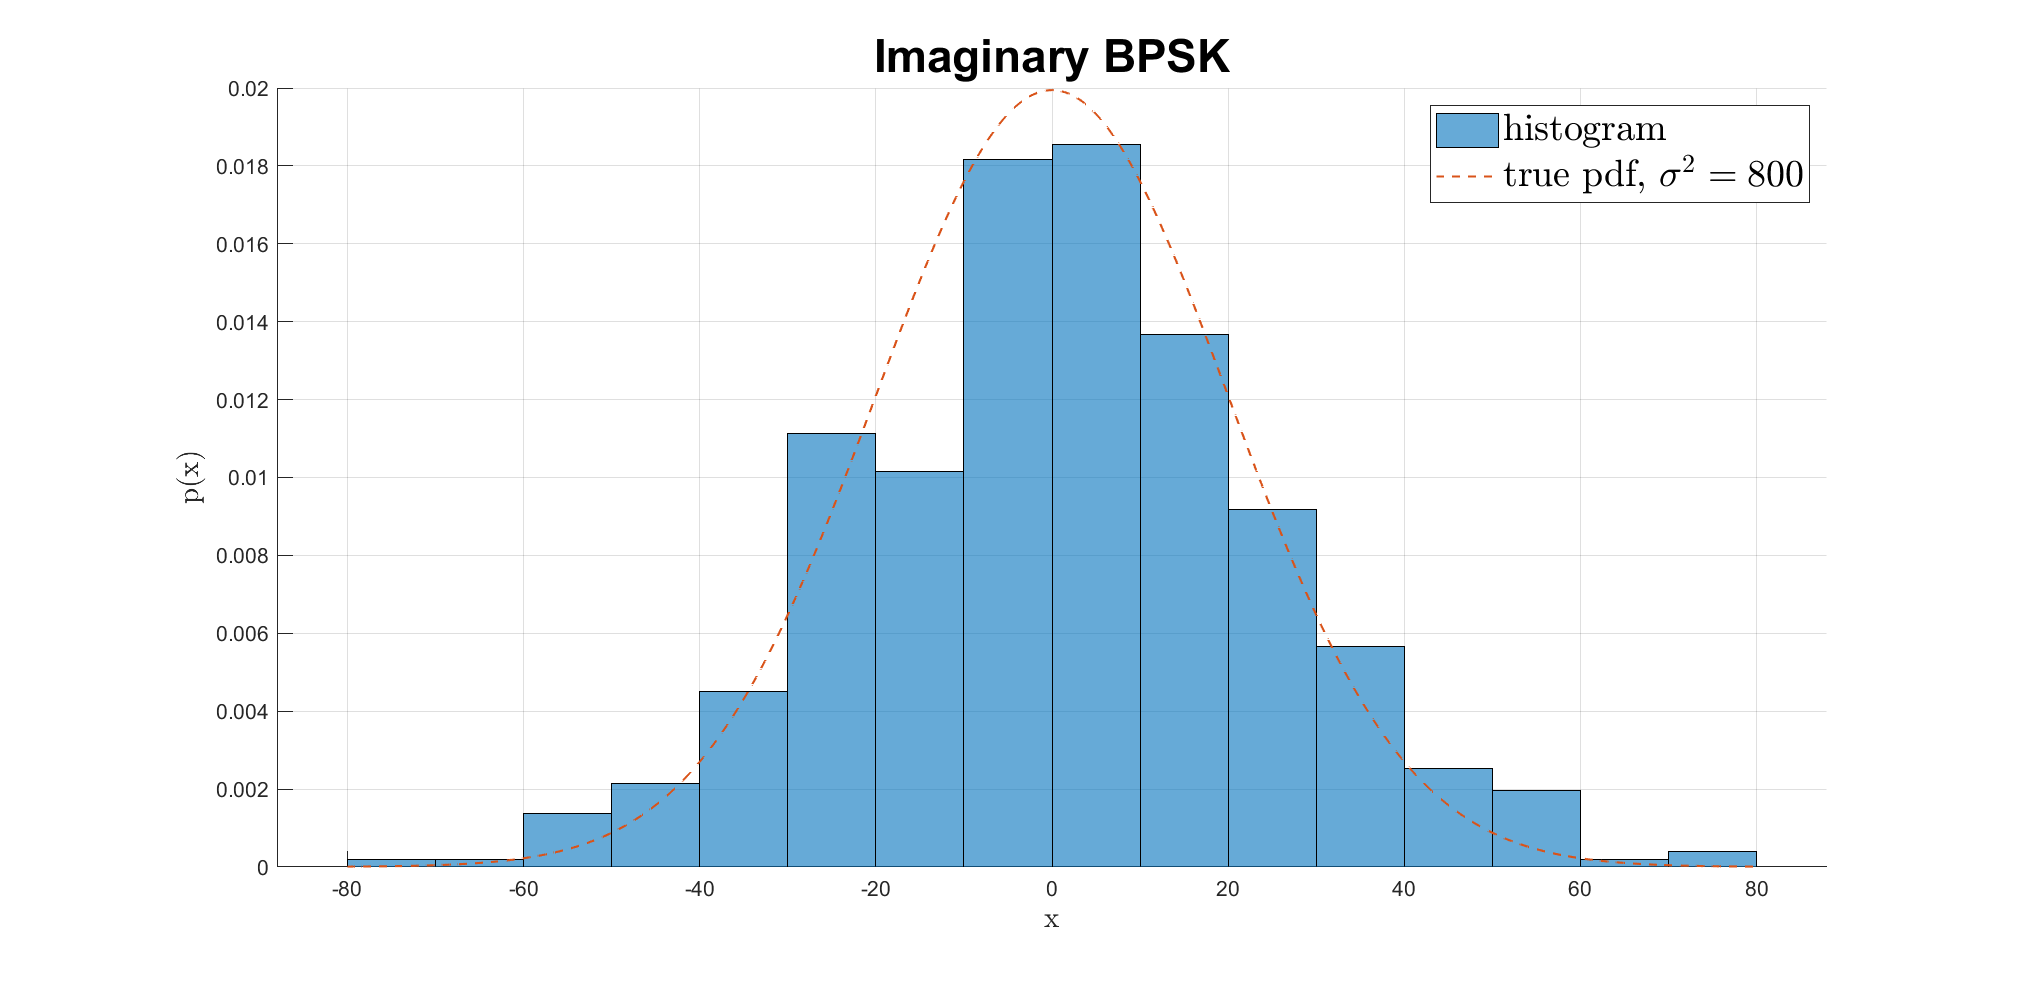
\includegraphics[width=.8\linewidth]{figures/im_bpsk.eps}
        \caption{The histogram of Im(S(k))$~$BPSK}
        \label{fig:im_bpsk}
    \end{subfigure}
    \caption{The histograms compared to pdf of gaussian}
    \label{fig:gauss}
\end{figure}
In the calculations of the variance and expected value for the four distributions the results were:
\begin{table}[ht]
\centering
\begin{tabular}{|l|l|l|l|}
\hline
\multicolumn{2}{|l|}{Gaussian} & \multicolumn{2}{|l|}{BPSK}\\ \hline
$\mathbb{E}\{s[n]$\} & $\mathbb{E}\{s_{r}[n]s_{i}[n]$\} & $\mathbb{E}\{s[n]$\} & $\mathbb{E}\{s_{r}[n]s_{i}[n]$\}\\
\hline
$0.53767-j2.0817\cdot10^{-16}$ & $1.707\cdot10^{-15}$ & $1-j6.5919\cdot10^{-17}$ & $2.4425\cdot10^{-15}$\\ 
\hline
\end{tabular}
\caption{Shows the expected value for each distributions}
\end{table}
However looking at the histogram it seems like the expected value is approximately at $0$ anyways for all the four distributions.
\subsection{Task 2: One-sample-detector}
In this task only one sample is used meaning that the detection problem is in this case:
\begin{align}
    H_0 &: x[0] = w[0]\nonumber\\
    H_1 &: x[0] = s[0]+w[0]\nonumber
\end{align}
It is given from the problem that $w\thicksim\mathbb{C}\mathcal{N}(0, \sigma_w^2)$ and $s\thicksim\mathbb{C}\mathcal{N}(\mu_s, \sigma_s^2)$ which means that under $H_0$, $x$ is from same distribution as $w$ and thus a complex gaussian with same mean and variance as $w$. Under $H_1$, which is a sum of two complex gaussian distribution, $x$ also is from a complex gaussian distribution. However the mean and variance needs to be calculated to adjust for both distributions.
The mean of $x[0]$ under $H_1$ is\todo{Usikker på om det er vits med disse utregningene}
\begin{align}
    \mathbb{E}\{x[0]\} & = \mathbb{E}\{s[0]+w[0]\}\nonumber\\
    & = \mathbb{E}\{s[0]\} + \mathbb{E}\{w[0]\}\nonumber\\
    & = \mu_s + 0 = \mu_s\nonumber
\end{align} 
The variance of $x[0]$ under $H_1$ is
\begin{align}
    \mathrm{Var}\{x[0]\} & = \mathrm{Var}\{s[0]+w[0]\}\nonumber\\
    & = \mathrm{Var}\{s[0]\} + \mathrm{Var}\{w[0]\}\nonumber\\
    & = \sigma_s^2+\sigma_w^2\nonumber
\end{align}
Meaning that
\begin{align}
    p(x;H_0) & = p_0(x) = \frac{1}{\sigma_w^2\pi}e^{-\frac{|x|^2}{\sigma_w^2}}\\
    p(x;H_1) & = p_1(x) = \frac{1}{(\sigma_w^2+\sigma_s^2)\pi}e^{-\frac{|x-\mu_s|^2}{\sigma_s^2+\sigma_w^2}}
\end{align}
Setting up the LRT:
\begin{align}
    L(x) & = \frac{p_1(x[0])}{p_0(x[0])} = \frac{\frac{1}{(\sigma_w^2+\sigma_s^2)\pi}e^{-\frac{|x[0]-\mu_s|^2}{\sigma_s^2+\sigma_w^2}}}{\frac{1}{\sigma_w^2\pi}e^{-\frac{|x[0]|^2}{\sigma_w^2}}}\nonumber\\
    & = \frac{\sigma_w^2}{\sigma_w^2+\sigma_s^2}e^{-\frac{1}{\sigma_w^2+\sigma_s^2}|x[0]-\mu_s|^2+\frac{1}{\sigma_w^2}|x[0]|^2}\nonumber
\end{align}
Since it is given that $\mu_s \approx 0$ this can be used to simplify the caluclations. The decision rule is to choose $H_1$ when $L(x[0]) \geq \lambda$, since $L(x[0])$ is a monotonically increasing function then the inequality holds for $\ln L(x[0]) \geq \ln\lambda$.
\begin{align}
    \ln L(x[0]) = \ln (\sigma_w^2)-\ln (\sigma_w^2+\sigma_s^2) & -\frac{1}{\sigma_w^2+\sigma_s^2}|x[0]|^2 +\frac{1}{\sigma_w^2}|x[0]|^2 \geq \ln\lambda\nonumber\\
    \left(\frac{1}{\sigma_w^2}+\frac{1}{\sigma_s^2+\sigma_w^2}\right)|x[0]|^2 & \geq \ln\lambda-\ln \frac{\sigma_w^2}{\sigma_w^2+\sigma_s^2}\nonumber\\
    |x[0]|^2 = x_R[0]^2+x_I[0]^2 & \geq \frac{\sigma_w^2(\sigma_w^2+\sigma_s^2)}{\sigma_s^2}\left(\ln\lambda-\ln\frac{\sigma_w^2}{\sigma_w^2+\sigma_s^2}\right) = \lambda'\nonumber
\end{align}
This also means that the decision rule is to choose $H_1$ when $|x[0]|^2\geq\lambda'$ and choose $H_0$ when $|x[0]|^2<\lambda'$ where
\begin{equation}
    \lambda' = \frac{\sigma_w^2(\sigma_w^2+\sigma_s^2)}{\sigma_s^2}\left(\ln\lambda-\ln \frac{\sigma_w^2}{\sigma_w^2+\sigma_s^2}\right)
\end{equation}\label{eq:lambda_prime}

\subsection{Task 3: Performance of the one-sample detector}
\begin{figure}[ht]
    \begin{subfigure}{.5\textwidth}
        \centering
        % include first image
        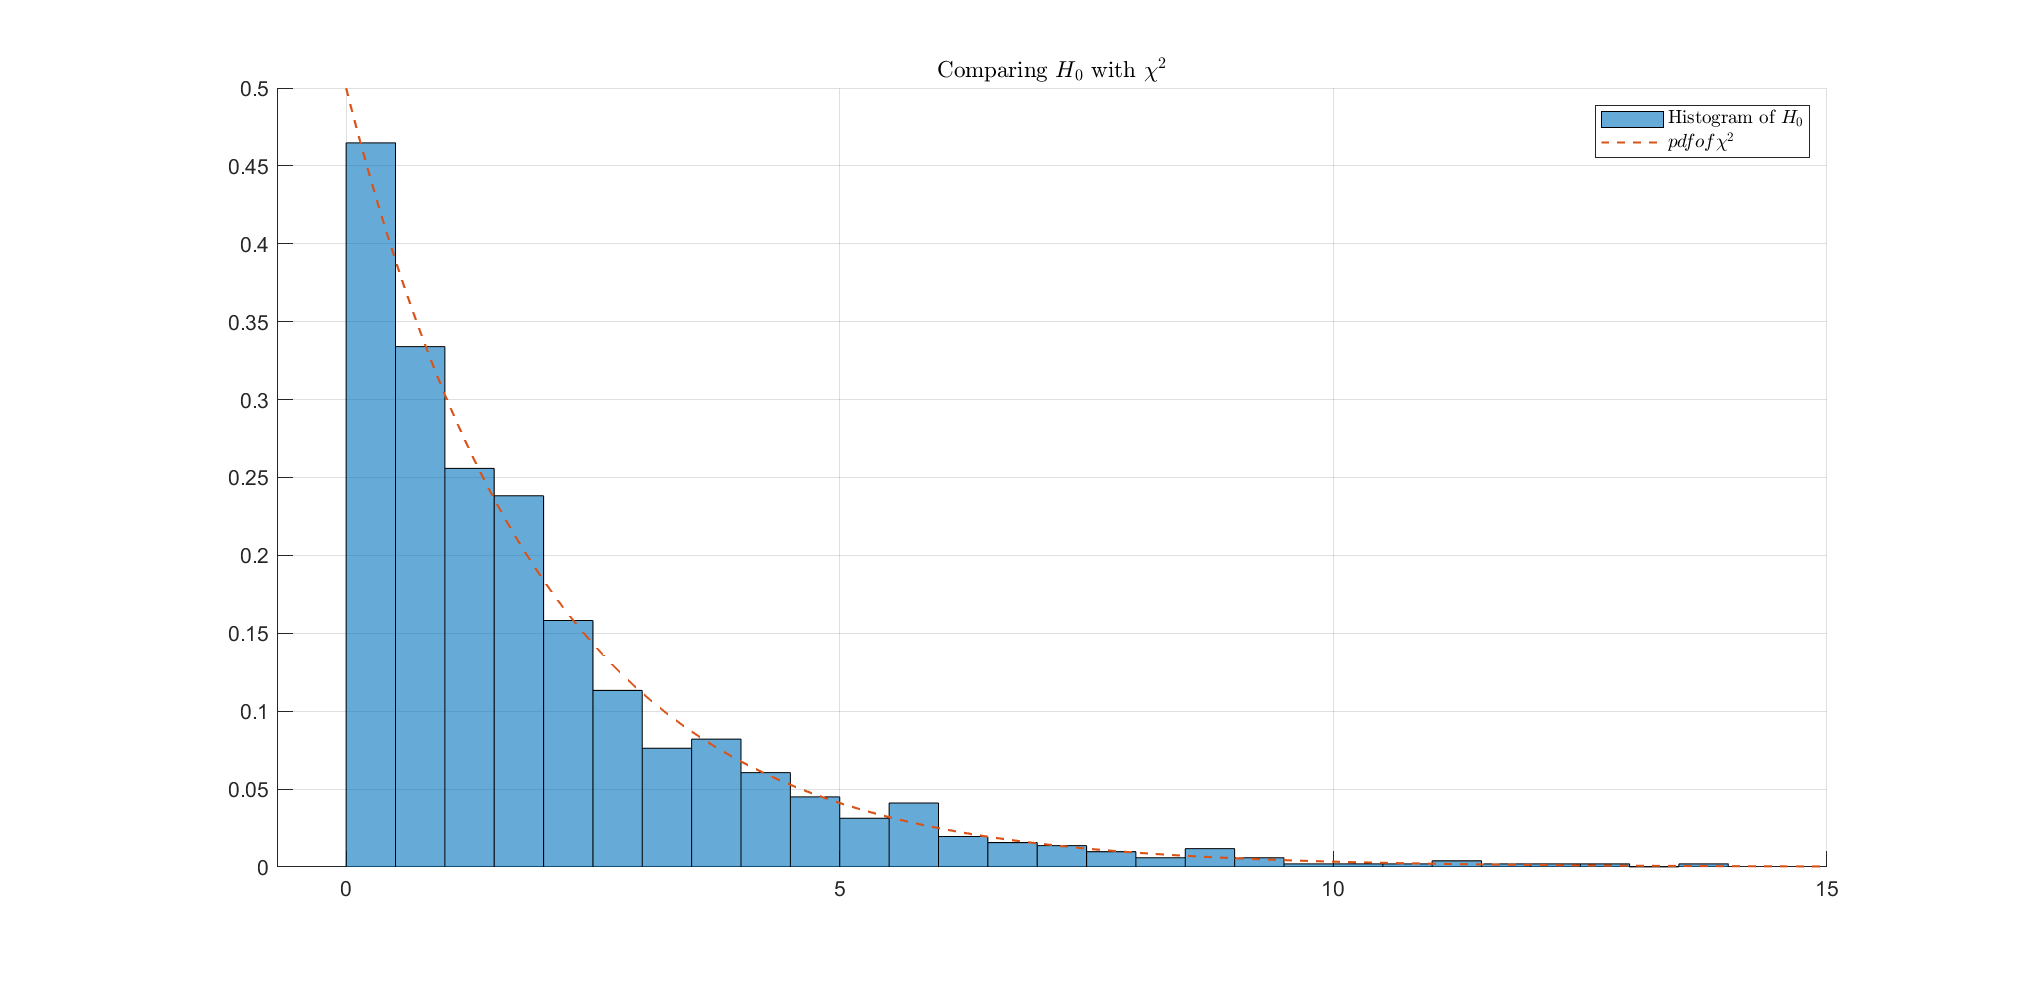
\includegraphics[width=.8\linewidth]{figures/chi_square_h0.eps}  
        \caption{The histogram of \eqref{eq:chi_sq_h0}}
        \label{fig:chi_sq_h0}
    \end{subfigure}
    \begin{subfigure}{.5\textwidth}
        \centering
        % include second image
        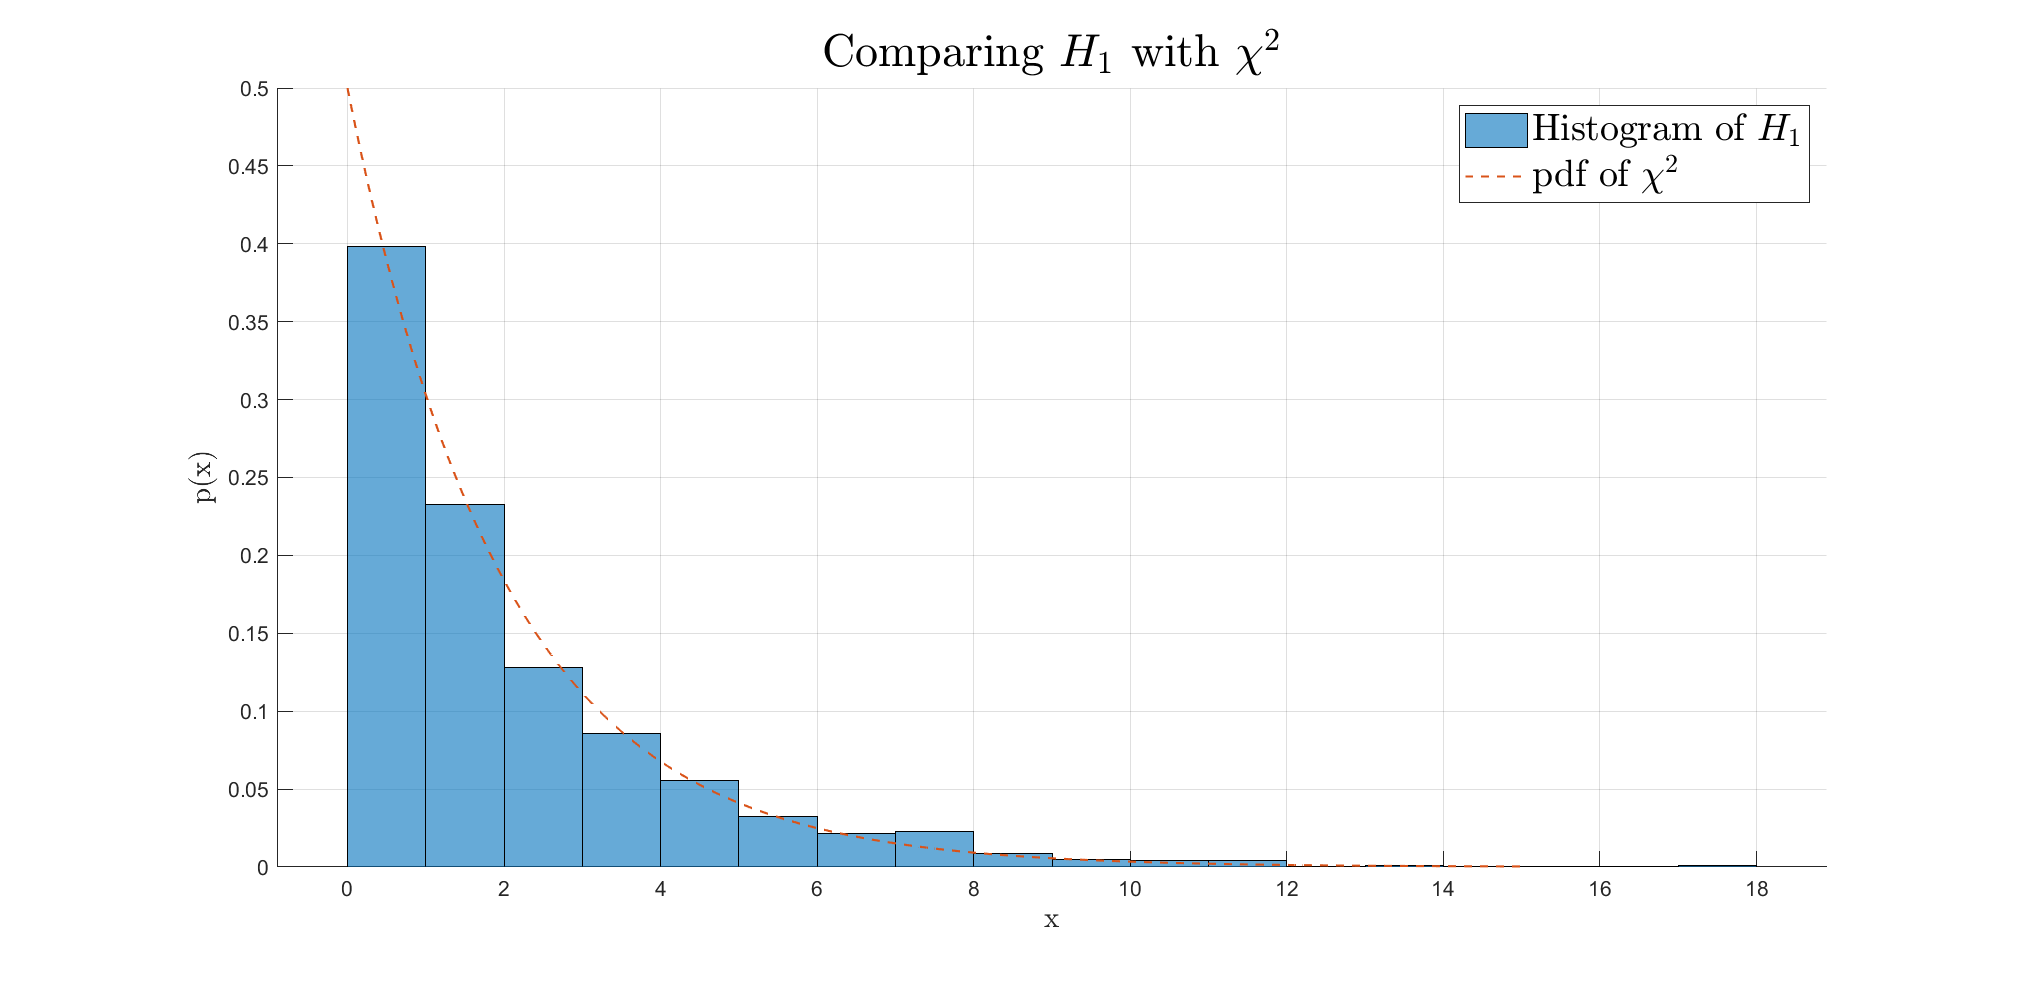
\includegraphics[width=.8\linewidth]{figures/chi_square_h1.eps}  
        \caption{The histogram of \eqref{eq:chi_sq_h1}}
        \label{fig:chi_sq_h1}
    \end{subfigure}
\end{figure}
The histogram in \ref{fig:chi_sq_h0} and \ref{fig:chi_sq_h1} shows that $|x[0]|^2$ is $\chi^2$-distributed with 2 degrees of freedom both under $H_0$ and $H_1$ and the difference between $H_0$ and $H_1$ is essentially the constant scaling factor given by the variances $\sigma_w^2$ and $\sigma_s^2$.
Calculating the probability for the false alarm gives
\begin{align}
    P_{FA} & = \text{Prob}\{|x[0]|\geq\lambda'\big\vert H_0\}\nonumber\\
    & = \int_{\lambda'}^{\infty}\frac{e^{-\frac{2x[0]}{2\sigma_w^2}}}{\sigma_w^2}dx[0]\nonumber\\
    & = -\frac{\sigma_w^2}{\sigma_w^2}e^{-\frac{x[0]}{\sigma_w^2}}\bigg\rvert_{\lambda'}^{\infty}\nonumber\\
    & = e^{-\frac{\lambda'}{\sigma_w^2}}\nonumber
\end{align}
Which only holds when $\lambda'>0$.\\
Furthermore the probability for detection is
\begin{align}
    P_D & = \text{Prob}\{|x[0]|\geq\lambda'\big\vert H_1\}\nonumber\\
    & = \int_{\lambda'}^{\infty}\frac{e^{-\frac{x[0]}{\sigma_w^2+\sigma_s^2}}}{\sigma_w^2+\sigma_s^2}dx[0]\nonumber\\
    & = -\frac{\sigma_w^2+\sigma_s^2}{\sigma_w^2+\sigma_s^2}e^{-\frac{x[0]}{\sigma_w^2+\sigma_s^2}}\bigg\rvert_{\lambda'}^{\infty}\nonumber\\
    & = e^{-\frac{\lambda'}{\sigma_w^2+\sigma_s^2}}\nonumber
\end{align}
Which also only holds for $\lambda'>0$\\

\subsection{Task 4: Generalized for multiple samples}
We take the one-sample-detector a step further and generalize it to use it for multiple samples. That is that the likelihood function is used to calculate the LRT so that we get
\begin{align}
    \ln L(x) & = \ln\prod_{n=0}^{K-1}\frac{1}{(\sigma_w^2+\sigma_s^2)\pi}e^{-\frac{|x(n)|^2}{\sigma_s^2+\sigma_w^2}}-\ln\prod_{n=0}^{K-1}\frac{1}{\sigma_w^2\pi}e^{-\frac{|x(n)|^2}{\sigma_w^2}}\nonumber\\
    & = \sum_{n=0}^{K-1}\left(\ln\frac{\sigma_w^2}{\sigma_w^2+\sigma_s^2} + \frac{|x(n)|^2}{\sigma_w^2}-\frac{|x(n)|^2}{\sigma_w^2+\sigma_s^2} \right)\nonumber\\
    & = \sum_{n=0}^{K-1}\left(\ln\frac{\sigma_w^2}{\sigma_w^2+\sigma_s^2} + \frac{\sigma_s^2}{\sigma_w^2(\sigma_w^2+\sigma_s^2)}|x(n)|^2\right)\geq\ln\lambda\nonumber
\end{align}
So the decision rule ends up being to choose $H_1$ when
\begin{equation}
    T(\mathbf{x}) = \sum_{n=0}^{K-1}|x(n)|^2 \geq \frac{\sigma_w^2(\sigma_w^2+\sigma_s^2)}{\sigma_s^2}\left(\ln\lambda-K\ln\frac{\sigma_w^2}{\sigma_w^2+\sigma_s^2}\right) = \lambda'
\end{equation}
Here $T(\mathbf{x})$ is a sum of $K$ complex Gaussian squared, meaning the pdf in this case is a $\chi^2$-distribution with $2K$ degrees of freedom. This means that
\begin{align}
    P_D & = \int_{\lambda'}^{\infty}\frac{x^{K-1}e^{-\frac{x}{\sigma_w^2+\sigma_s^2}}}{(\sigma_w^2+\sigma_s^2)^K\Gamma(K)}dx\nonumber\\
    & = \frac{1}{(\sigma_w^2+\sigma_s^2)^K\Gamma(K)}\int_{\lambda'}^{\infty}x^{K-1}e^{-\frac{x}{\sigma_w^2+\sigma_s^2}}dx\nonumber\\
    & = \frac{1}{\sigma_w^2+\sigma_s^2}Q\left(\frac{\lambda'}{\sigma_w^2+\sigma_s^2}\right)
\end{align}
Differentiating the integral with respect to $\lambda'$ it shows that $P_D$ is strictly decreasing and has extremal points at $\lambda'=0\vee\lambda'=\infty$. Which essentially means that $P_D$ is maximized when $\lambda'\in[0,\infty)$ is as close to $0$ as possible. For the false alarm with the upper limit $\alpha_0$, its cumulative distribution function is
\begin{align}
    P_{FA} & = \frac{1}{(\sigma_w^2)^K\Gamma(K)}\int_{\lambda'}^{\infty}x^{K-1}e^{-\frac{x}{\sigma_w^2}}dx\nonumber\\
    & = \frac{1}{\sigma_w^2}Q\left(\frac{\lambda'}{\sigma_w^2}\right) \leq \alpha_0
\end{align}

Which means that for the inequality to hold in addition to maximize the power of the test, need to choose $\lambda' >= \sigma_w^2Q^{-1}\left(\alpha_0\right)$. Essentially choosing $\lambda' = \sigma_w^2Q^{-1}\left(\alpha_0\right)$ to minimize $P_D$. Inserting this to get the expression for $P_D$.
\begin{equation}
    P_D = \frac{1}{\sigma_w^2+\sigma_s^2}Q(\frac{\sigma_w^2}{\sigma_w^2+\sigma_s^2}Q^{-1}\left(\alpha_0\right))
\end{equation}

\subsection{Task 5: }
As mentioned in the task before, 

\subsection{Task 6: Central limit theorem}
By the central limit theorem that states that for $T(\mathbf{x}) = \sum_{n=0}^{K-1}|x[n]|^2$, that $T(\mathbf{x})$ converges to a Gaussian distribution when $|x[n]|^2$ comes from a independent identical distribution with finite expected value $\mu$ and finite variance $\sigma^2$. Already know that $|x[n]|$ is complex gaussian and iid for each sample $n = 0, \dots, K-1$ so $|x[n]|^2$ is also iid.\\
\begin{figure}
    \centering
    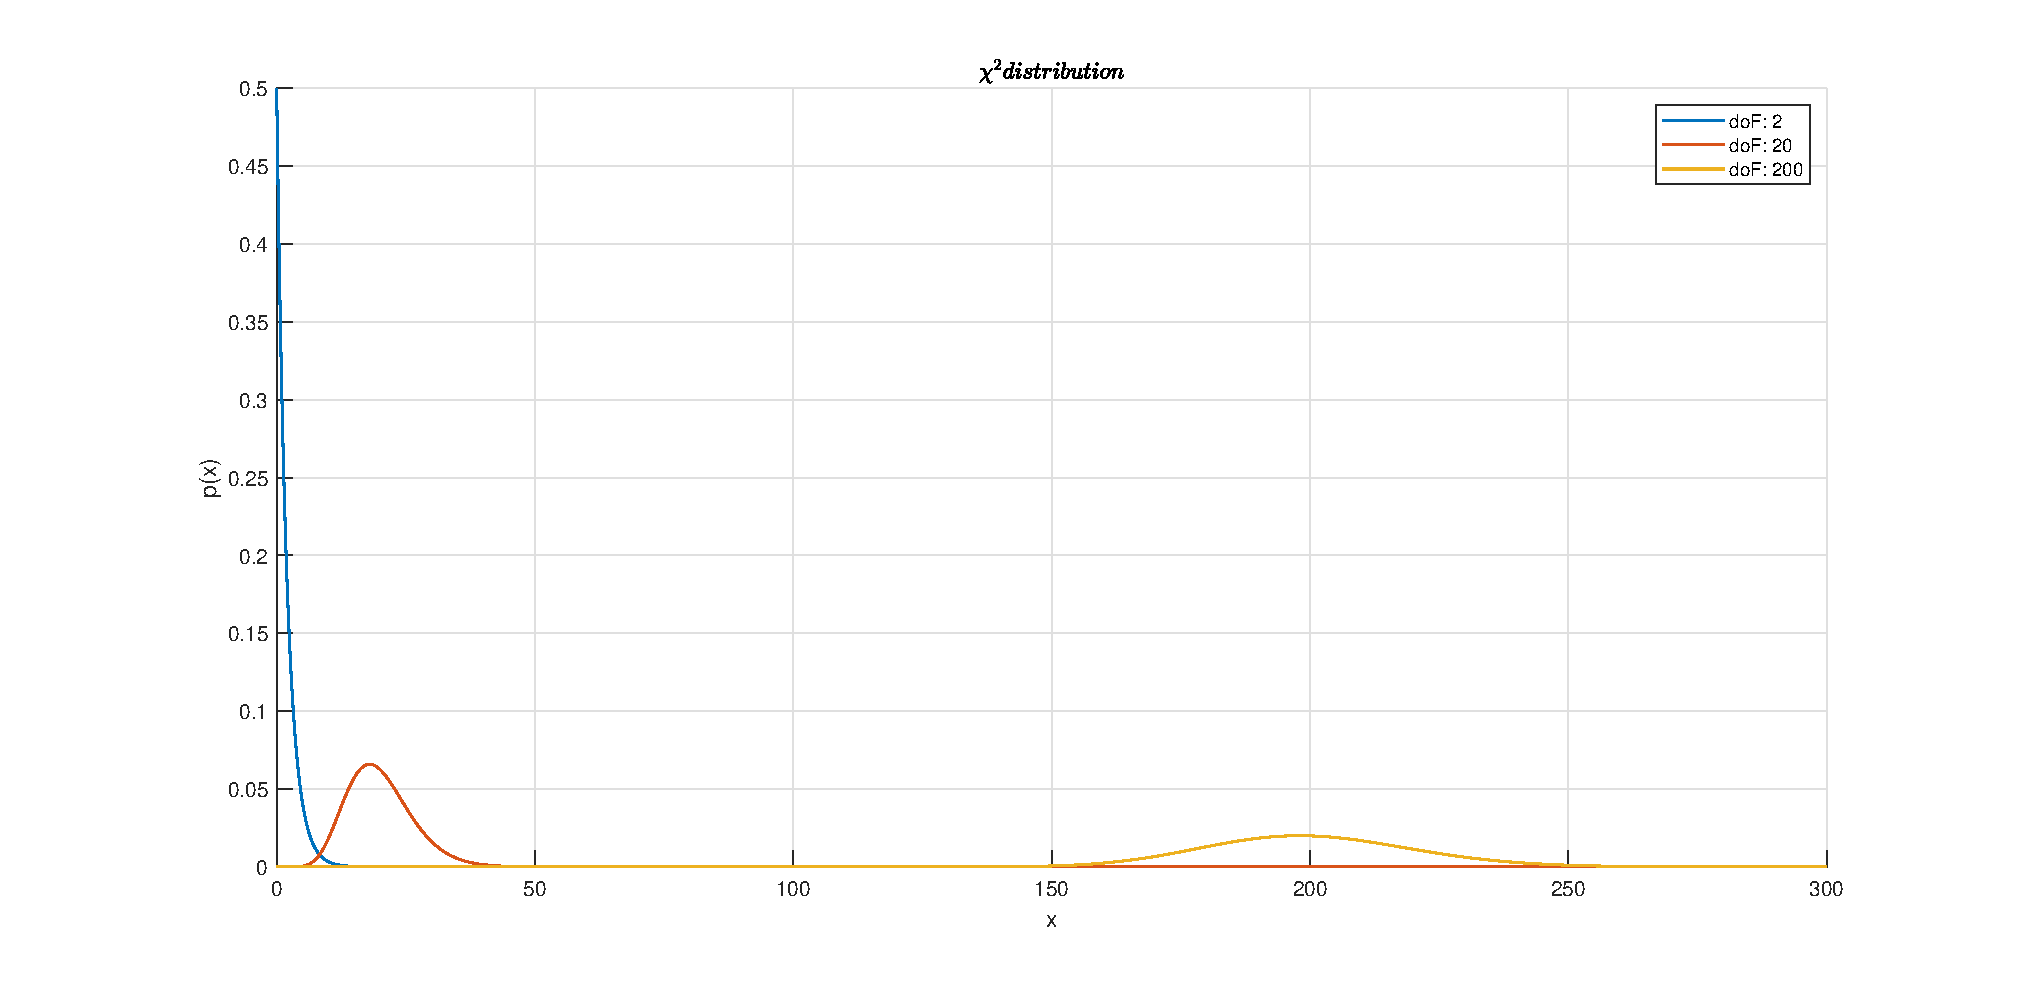
\includegraphics[width=\textwidth]{figures/chi_square}
    \caption{Caption}
    \label{fig:my_label}
\end{figure}
In this case the mean is
\begin{align}
    \mathbb{E}\left\{T(\mathbf{x})\right\} & = \mathbb{E}\{\sum_{n=0}^{K-1}|x[n]|^2\}\nonumber\\
    & = \sum_{n=0}^{K-1}\mathbb{E}\{|x[n]^2|\} = \hat{\mu}
\end{align}
and the variance is
\begin{align}
    \mathrm{Var}\left\{T(\mathbf{x})\right\} & = \mathrm{Var}\{\sum_{n=0}^{K-1}|x[n]|^2\}\nonumber\\
    & = \sum_{n=0}^{K-1}\mathrm{Var}\{|x[n]^2|\} = \hat{\sigma}^2
\end{align}
Which gives the pdf of a normal gaussian
\begin{equation}
    f(x) = \frac{1}{\sqrt{2\pi\hat{\sigma}^2}}e^{-\frac{1}{2}\left(\frac{x-\hat{\mu}}{\hat{\sigma}^2}\right)^2}
\end{equation}







\subsection{Task 7: How many samples do we need for it to be good enough}

\subsection{Task 8: Test with data}

\begin{enumerate}[i]
    \item What is this chapter about
    \item Matlab implementation
    \item Any specific Matlab m-commands used?
    \item A flow-diagram is recommended
    \item Results (use figures/tables if possible)
    \item Discussion of results
    \item Matlab code (documented) in appendix
\end{enumerate}






\section{Conclusion}\label{sec:conclusion}
This project focused on Spectrum Sensing in OFDM Cognitive Radios, which is an important problem in modern communication as the spectrum is a scarce resource. After modeling how the signal data was generated, a suitable detector for the binary hypothesis testing was implemented. This was a result of using well known statistical features of the Gamma and Gaussian distribution, as well as the Neyman-Person Lemma. After testing the performance of the one-sample-detector, a more generalized K-sample detector was implemented. This new NP detector for K samples was then approximated as a Gaussian random variable which showed to be quite accurate to the original gamma distribution. This detector based on K samples showed to be useful in the way that one could choose a $P_{D}$ and $P_{FA}$ only at the cost of more samples K. In the end, this whole detector was put to a test when a data set of 100 realizations of a signal from a PU was tested on the detector. As the result in task 8 have shown, the detector did very well, and detected the signal almost every time, however increasing K manually gave a detection rate of $100\%$.\\
The project has been very educational and it has been specifically interesting to see how probability distributions are used in modern communications systems for hypothesis testing. With an increasing number of communication devices this problem is highly relevant.



\newcommand{\texMacro}[2]{\texttt{\textbackslash{#1}\{#2\}}}
\section{General LaTeX tips}\label{sec:latex_tips}
Some tips were given in \Cref{sec:intro}, and this section will elaborate with some more concrete examples. Also check out the source files for some additional useful packages.

\subsection{Matrix Equations}
Here is a matrix equation you can use as a template:
\begin{equation}
	\begin{bmatrix}
		1 &  0 &  0 & 0 & -b &  0 &  0 &  0 \\
		-a &  1 &  0 & 0 &  0 & -b &  0 &  0 \\
		0 & -a &  1 & 0 &  0 &  0 & -b &  0 \\
		0 &  0 & -a & 1 &  0 &  0 &  0 & -b                                
	\end{bmatrix}
	\begin{bmatrix} x_1 \\ x_2 \\ x_3 \\ x_4 \\ u_0 \\ u_1 \\ u_2 \\ u_3 \end{bmatrix}
	=
	\begin{bmatrix}
		ax_0 \\ 0 \\ 0 \\ 0      
	\end{bmatrix}
\end{equation}

\subsection{Tables}
If you want, you can use the source for \Cref{tab:parameters} to see how a (floating) table is made. Variables and symbols are always in italics, while units are not. Generating large, complicated tables can get very tedious. Luckily there exists some tools that can assist the table generation, see e.g. \url{http://www.tablesgenerator.com/}.



\begin{table}[tbp]
	\centering
	\caption{Parameters and values.}
	\begin{tabular}{llll}
		\toprule
		Symbol & Parameter & Value & Unit \\
		\midrule
		$l_{c}$     & Distance from elevation axis to counterweight   & $0.50$  & \meter                      \\
		$l_{h}$     & Distance from elevation axis to helicopter head & $0.64$  & \meter                      \\
		$l_{p}$     & Distance from pitch axis to motor               & $0.18$  & \meter                      \\
		$K_f$       & Force constant motor                            & $0.25$  & \newton\per\volt            \\
		$J_e$       & Moment of inertia for elevation                 & $0.83$  & \kilogram\usk\meter\squared \\
		$J_\lambda$ & Moment of inertia for travel                    & $0.83$  & \kilogram\usk\meter\squared \\
		$J_p$       & Moment of inertia for pitch                     & $0.034$ & \kilogram\usk\meter\squared \\
		$m_h$       & Mass of helicopter                              & $1.05$  & \kilogram                   \\
		$m_{p}$     & Motor mass                                      & $1.81$  & \kilogram                   \\
  		$m_{c}$     & Counterweight mass                              & $0.73$  & \kilogram                   \\
		\bottomrule
	\end{tabular}
\label{tab:parameters}
\end{table}

\subsection{The \texMacro{input}{} command}
By using \texMacro{input}{whatever} in your main tex file (\texttt{labreport.tex} in this case), the content of \texttt{whatever.tex} will be included in your pdf. This way you can split the contents into different files, e.g.~one for each problem of the assignment. This makes it easier to restructure the document, and arguably improves the readability of the tex files. For instance; maybe you want each problem to start on a new page? Simply add \textbackslash{newpage} before each \texMacro{input}{} command. Alternatively, you can use the \texMacro{include}{} command to achieve more or less the same effect. See~\cite{InputVsInclude} for more information.

\subsection{Citations and Reference Management}
In academic writing, it is very important to cite your sources. In Latex this is done by defining an an entry in a \emph{BibTeX} bibliography file like this (from \texttt{bibliography.bib}):
\lstinputlisting[language=Tex, firstline=1, lastline=7]{bibliography.bib}
and then using the \texttt{\textbackslash{cite}} command in your Latex document. For instance \texttt{\textbackslash{cite}\{Chen2014\}} will produce~\cite{Chen2014}.

There are many different citation styles, and a lot of customization that is possible, so please check out e.g.~\cite{BiberBibtexEtc,WikibookLatex}\footnote{Keep citation of web pages to a minimum, and consider using \url{http://web.archive.org} if you are worried that the reference may change or be removed in the future.}.

There is also a lot of useful software to manage your references. Some popular examples include JabRef (\url{http://www.jabref.org/}), Mendeley (\url{https://www.mendeley.com/}) and EndNote. JabRef is perhaps the simplest of these three, and stores all information in a \texttt{.bib} file that you can directly use in your Latex document. Both Mendeley and EndNote can export references as BibTeX.

\subsection{listings}
 The \texttt{listings} package makes it easy to include code in the report. For example \cref{lst:label} includes code that is written in the tex file. You can also specify what the code listings should look like: color, line numbers, frames\ldots
 
 \begin{lstlisting}[caption={Some Matlab code, with the source in the tex file},label={lst:label},language=Matlab, float]
   degree = 6;
   out = ones(size(X1(:,1)));
   for i = 1:degree
      for j = 0:i
	 out(:, end+1) = (X1.^(i-j)).*(X2.^j);
      end
   end
 \end{lstlisting}
% Uncomment the following line to take the code directly from the source file 'some_function.m'
 %\lstinputlisting[language=Matlab, firstline=4, lastline=10, caption={Another piece of code, directly from the source file}, label={lst:listing2},float]{some_function.m}
 This is great! However, try to keep the amount of code in the report to a reasonable level, and remember; code in itself is not an explanation.
 
 %See \url{http://ctan.mirrors.hoobly.com/macros/latex/contrib/listings/listings.pdf} for more information.
 
 \subsection{todonotes}
 The \texttt{todonotes} package is great for work in progress. Few things are more embarrassing than forgetting to remove ``Remember to fix this before delivery!!!!!!'' from the middle of your report. Instead, use \texttt{\textbackslash{todo}\{Remember to fix this before delivery!!!!!!\}} \todo{Remember to fix this before delivery!!!!!!}. This will show up like a red box in the margin. Some prefer \texttt{\textbackslash{todo}{[inline]}\{FIXME2!!!\}} which produces \todo[inline]{FIXME2!!!} %since the todos in the margin tend to cause 'Overfull \hbox' warnings.

 %To avoid typing [inline] all the time, you can define  
 %\newcommand{\TODO}[1]{\todo[inline]{#1}}
 %in the preamble of the document, and then use \TODO
You can also use \textbackslash{listoftodos} to get a list of all the todos in your document, and \textbackslash{missingfigure} will create a dummy figure, like \cref{fig:my_awesome_fig}, that you can replace once you have made a proper figure. This way you can start referencing figures/plots before you make them, and still be reminded that you need to make them.

 \begin{figure}[h]
   \centering
   \missingfigure{Plot of pitch and desired pitch from problem 1.2.3}
   \caption{Pitch and desired pitch}
   \label{fig:my_awesome_fig}
\end{figure}
 
When you are finished with your report (or have run out of time) you can simply change \textbackslash{usepackage}\{todonotes\} to \textbackslash{usepackage}[disable]\{todonotes\} and they will all magically disappear!
%See \url{http://ctan.math.utah.edu/ctan/tex-archive/macros/latex/contrib/todonotes/todonotes.pdf} for more information. 

\subsection{cleveref}
The observant reader might have noticed the use of \texttt{\textbackslash{cref}} in referencing tables, figures etc. This is a bit more clever than the normal \texttt{\textbackslash{ref}} because it detects what you are referencing based on the prefix of the label. Then it prints the appropriate ``prefix''. So \texttt{\textbackslash{cref}\{fig:my\_awesome\_fig\}} will produce \cref{fig:my_awesome_fig}, whereas \texttt{\textbackslash{cref}\{tab:parameters\}} will produce \cref{tab:parameters}. Notice how the labels of the table and the figureare prefixed with \texttt{tab:} and \texttt{fig:} respectively. If you want it to say e.g. ``figure'' instead of ``fig.'', this is completely customizable. There is also \texttt{\textbackslash{Cref}} for a capitalized version.


% References
\newpage
\addcontentsline{toc}{section}{References}
\printbibliography{}
\label{sec:bibliography}

% appendix of matlab codes
\addcontentsline{toc}{section}{Appendix} % Remove this if you don't want the appendix included in the table of contents.
\appendix
\section{MATLAB code}
\subsection{Problem 1}
\lstinputlisting{code/problem1.m}
\subsection{Problem 3}
\lstinputlisting{code/problem3.m}
\subsection{Problem 5}
\lstinputlisting{code/problem5.m}
\subsection{Problem 6}
\lstinputlisting{code/problem6.m}
\subsection{Problem 8}
\lstinputlisting{code/problem8.m}
% \input simply inserts the contents of the file, while \include forces a \newpage.
% See \input vs. \include: http://tex.stackexchange.com/questions/246/when-should-i-use-input-vs-include

\end{document}
